\section{Sicurezza}
In questa sezione verranno descritti i meccanismi di autenticazione e autorizzazione scelti per
garantire un adeguato livello di sicurezza agli utenti.

\subsection{Autenticazione}
L'autenticazione è un metodo che permette l'identificazione degli utenti sulla base di un set di credenziali e
verificare che questi forniscano le giuste informazioni per accedere alla applicazione.

L'implementazione presente all'interno della piattaforma si basa su una coppia di credenziali: email e password.
Per garantire una archiviazione sicura delle password è stato deciso di applicare una policy basata sull'uso di \textit{hash} e \textit{salt}.


- spiegazione di hash -
- spiegazione di salt -
- che problema risolve la loro introduzione -


\subsection{Autorizzazione}
L'autorizzazione è un metodo che permette di garantire la riservatezza e la disponibilità dei dati.
Attraverso l'implementazione di policy è infatti possibile definire dei protocolli che permettono di restringere l'accesso alle risorse,
rendendole disponibili solo agli utenti autorizzati.

Le policy definite all'interno della piattaforma si basano sul protocollo di autorizzazione OAuth 2.0 \cite{rfc6749} e sull'utilizzo di un
modello di controllo sugli accessi basato sui ruoli dei singoli utenti.


\subsubsection{OAuth 2.0}
OAuth 2.0 \cite{rfc6749} è un framework autorizzativo standard per applicazioni Web.
Scopo del framework è delegare a un'utenza qualsiasi l'accesso limitato a una risorsa di proprietà di un'entità differente (detta \textit{resource owner}).

Gli attori coinvolti nell'architettura del framework sono:
\begin{itemize}
    \item \textit{Resource Owner}: il proprietario della risorsa esposta. Può essere una applicazione o un utente.
    \item \textit{Resource Server}: è il server che detiene la risorsa esposta.
    \item \textit{Authorization Server}: è il server o il modulo applicativo che rilascia i token di accesso (detti \textit{access token}) al client dopo aver
          autenticato con successo il \textit{resource owner} e aver ottenuto l'autorizzazione.
    \item  \textit{Client}: è l'applicazione che richiede l'accesso alla risorsa. Può essere sia una applicazione \textit{client-side} che \textit{server-side}.
\end{itemize}

Altri elementi significativi sono l'\textit{access token} e l'\textit{authorization grant}.
Il primo è una stringa che rappresenta le credenziali necessarie per ottenere l'accesso alla risorsa protetta sul resource server.
Pratica comune è utilizzare il formato Json Web Token\cite{rfc7519} (JWT) che permette di codificare un oggetto JSON in un token
che può essere cifrato e firmato con vari algoritmi (HMAC, RSA, ECDSA). Questo permette di trasmettere in modo sicuro e compatto delle informazioni
fra due interlocutori garantendone integrità e confidenzialità.
L'\textit{authorization grant} rappresenta le credenziali che verificano l'autorizzazione fornita dal \textit{resource owner} e usate dal \textit{client} per ottenere un \textit{access token}.
Il framework ne definisce quattro tipologie: \textit{authorization code}, \textit{implicit}, \textit{resource owner password credentials} e \textit{client credentials}.

Il processo di base definito dal protocollo per autenticare il client e fornire un \textit{access token} è il seguente:
\begin{figure}[h]
    \centering
    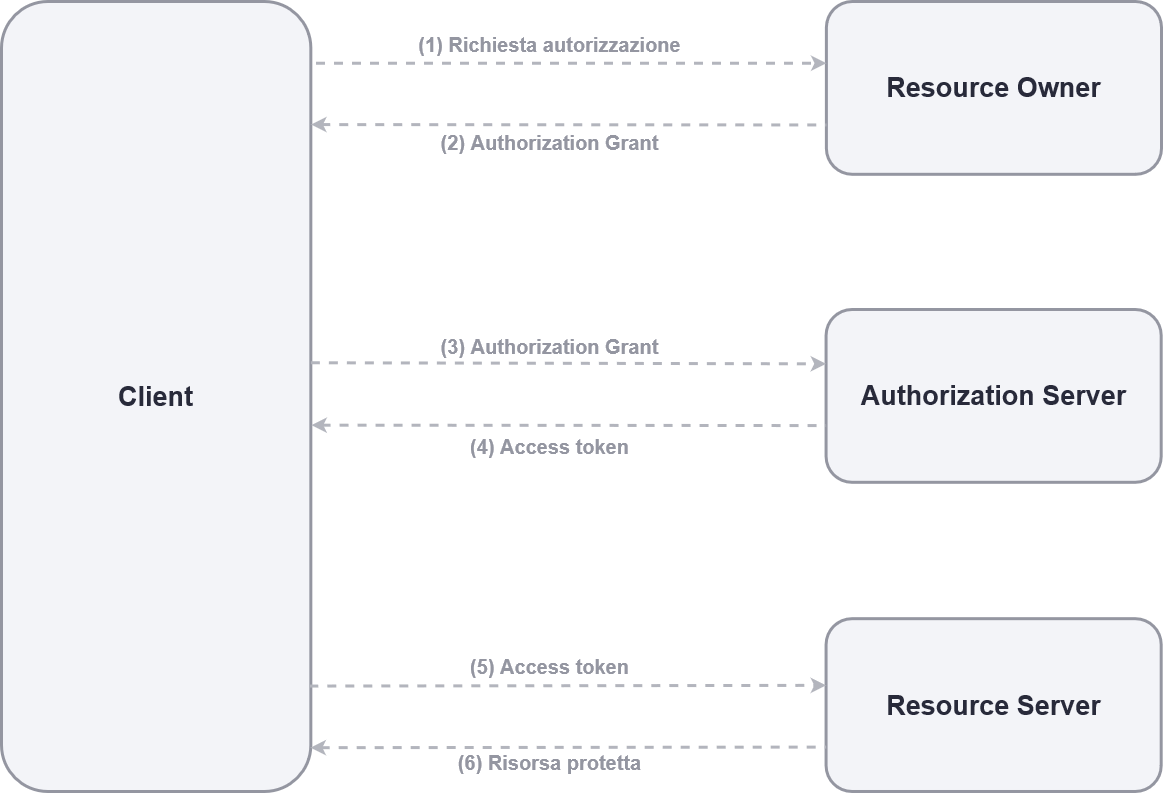
\includegraphics[width=0.75\textwidth]{oauth.png}
    \caption{Flusso del protocollo OAuth 2.0}
    \label{fig:OAuth2.0}
\end{figure}

\begin{enumerate}
    \item Il \textit{client} richiede l'autorizzazione al \textit{resource owner}.
    \item Il \textit{client} riceve un \textit{authorization grant}, ovvero delle credenziali che rappresentano l'autorizzazione del \textit{resource owner}.
    \item Il \textit{client} richiede un \textit{access token} autenticandosi con l' authorization server e fornendo l'\textit{authorization grant}.
    \item L'\textit{authorization server} autentica il client validando l'\textit{authorization grant}. Se è valido fornisce un \textit{access token}.
    \item Il \textit{client} richiede l'accesso alla risorsa protetta presente nel \textit{resource server} e si autentica presentando l'\textit{access token}.
    \item Il resource server valida l'\textit{access token} e, se è valido, gestisce la richiesta.
\end{enumerate}



nella piattaforma è stato usato quello X per fare Y.
Inoltre viene utilizzato il meccanismo del refresh token e dell'access token per questi motivi.

